\chapter{Calcium Data of T Cells}
\label{chapter:data}

From section~\ref{sec:t-cell/activation}, we gather that analysing the intracellular \Calcium concentration gives us good insight in whether and when a cell activates. Additionally, it can be measured relatively easily by the method described in this chapter.

\section{Structure of the Data}
\label{sec:structure_of_data}

First we describe the structure of the data this work uses. 

The data matrix has one row for each combination of tracked particle and frame number. In this context cells are called particles as the recording might feature non-cells that are detected as a cell and recorded in the data set. The information stored for each particle and frame combination is described in detail in table~\ref{tab:information_data_matrix}.

\begin{table}[h!]
	\centering
	\begin{tabular}{|c|c|l|}
		\hline
		\textbf{Name} & \textbf{Data Type} & \textbf{Description} \\
		\hline
		x & float64 & Position of particle in pixels along the horizontal axis \\
		\hline
		y & float64 & Position of particle in pixels along the vertical axis \\
		\hline
		frame & int32 & Number of frame, with frame rate of 1 frame per second \\
		\hline
		mass short & float64 & Brightness of cell in 340nm channel \\
		\hline
		%bg short & float64 & Background in 340nm channel \\
		%\hline
		mass long & float64 & Brightness of cell in 380nm channel \\
		\hline
		%bg long & float64 & Background in 380nm channel \\
		%\hline
		ratio & float64 & Calculated as mass short divided by mass long \\
		\hline
		particle & int32 & Identification for each particle \\
		\hline
	\end{tabular}
	\caption{Description and data type of all columns present in the data matrix.}
	\label{tab:information_data_matrix}
\end{table}

% mouse pos: 4289, 720; mouse neg: 7683, 785; human pos: 694, 948

One recording can have between 500 and 10000 particles and is between 700 and 1000 frames long, which corresponds to between about 11 and 17 minutes. The ratio recorded is typically between 0 and 5.

Four recordings where generated, with two each from human and mouse cells. For each cell type a positive and negative control was measured. In a positive control the conditions are such, that in theory every cell should activate, while in negative control the conditions are such, that none should activate. Due to stress on the cells caused by the movement or changes in temperature and other factors a few cells will activate before the recording starts, during the recording in the negative control or not activate at all in the positive control, regardless of the conditions.

\section{Jurkat Cells, 5c.c7 Primary Mouse T Cells and Fura-2}

The prototypical cell line to study T cell signalling is the Jurkat cell line.\cite{morgan2023} It was obtained from the blood of a boy with T cell leukaemia.\cite{schneider1977} Different cell lines within the Jurkat family are described by Abraham and Weiss.\cite{abraham2004} They provide a timeline of discoveries linked to Jurkat cells and t cell receptor signalling. Another type of t cells used in signalling studies are gathered from mice.

In order to be able to measure the intracellular \Calcium concentration of cells they can be labelled with Fura-2. This method provides a way to record the \Calcium concentration of multiple cells over a time period.\cite{martinez2017} Challenges encountered when using Fura-2 on certain cell types are described by Roe, Lemasters and Herman along with their respective solutions.\cite{roe1990}

\section{Measuring the Calcium Concentration of T Cells}

After the cells have been labelled with Fura-2, a recording of up to 15 to 20 minute can be generated. To achieve this the cells and stimulant are photographed at both 340nm and 380nm wavelength once per second. The resolution of the images are 1.6um per pixel. By calculating the ratio of the two images at each pixel the \Calcium concentration can be observed. An exemplary resulting image showing the ratio is shown in figure~\ref{fig:example_ratio_img}. The T cells appear a lighter shade than the background when activated and darker when not activated.

\begin{figure}
	\centering
	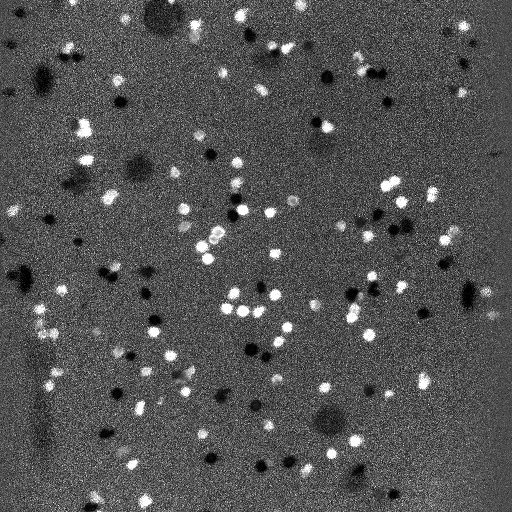
\includegraphics[width=0.6\linewidth]{fig/frame_ratio.jpg}
	\caption{Single frame showing the ratio of the 340nm and 380nm images from a recording of human Jurkat cells. Activated cells appear lighter, unactivated cells darker than the background. Big dark circles are out of focus cells that have not yet settled on to the plate.}
	\label{fig:example_ratio_img}
\end{figure}

To activate the cells in the duration of the recording they are transferred to a plate covered with replicas of the MHC-peptide complex normally present on APCs. This plate is then recorded as described above. For a negative control the plate is not covered with peptides, while for the positive control the peptide covering on the plate is very dense. Recordings of different densities in peptides lead to activation of a percentage of t cells.

\section{Processing the Data}

To track single t cells moving around during the video the sum of the 340nm and 380nm image of each second is calculated. This image provides the basis for separating t cells from the background. On this image all t cells will appear similarly light in colour. Therefore, it is used to track the movement of cells. Each cell is numbered, such that the same cell will have the same number during the video. For some cells the trajectory tracking is not perfect, resulting in a split of the numbering into multiple numbers for the same cell. The position and shade during both 340nm and 380nm as well as the ratio of each particle and each frame is then recorded into the data structure used in this work. The first roughly 50 frames at the start of the recording are discarded due to the video being out of focus. Additionally, cells only appearing in fewer than 300 frames are discarded as they most likely represent trajectories incorrectly tracked or split. The resulting data is then stored in a matrix structured as described in table~\ref{tab:information_data_matrix}.
